% vim: set tw=78 sts=2 sw=2 ts=8 aw et ai:
With the goal of comprehending the traffic policies employed by Operator 1, we
have run tests between our Galaxy Nexus I9250 and our public server. Tests
have run every 30 minutes over the span of 24 hours, recording both upload and
download throughputs. Additionally, we have alternated between CUBIC and OLIA
as congestion control algorithms. The reason we have looked into these
features is that we would like to derive an accurate image of the manner in
which Operator 1 handles traffic passing through its network.

Prior to launching these longterm tests, we have established a baseline during
daytime hours, for comparison purposes. We have managed to reach throughput of
roughly 4Mbps, for both upload and download. This particular operator
advertises maximum speeds of 150Mbps for download and 75Mbps for upload.

Initially we have used CUBIC, the default congestion control algorithm used
on Linux systems, which is not designed to be aware of multiple paths. In
terms of upload, Figure \ref{fig:up-cubic} highlights that throughput reaches values
of up to 14Mbps, but averages aroung 8Mbps. While there are some spontaneous
drops, more prolonged periods of lower throughput can be noticed in the
morning, before noon, and in the evening, after 20:00. This can be correlated
with devices being used before and after work hours, respectively.

\begin{figure}[H]
  \centering
  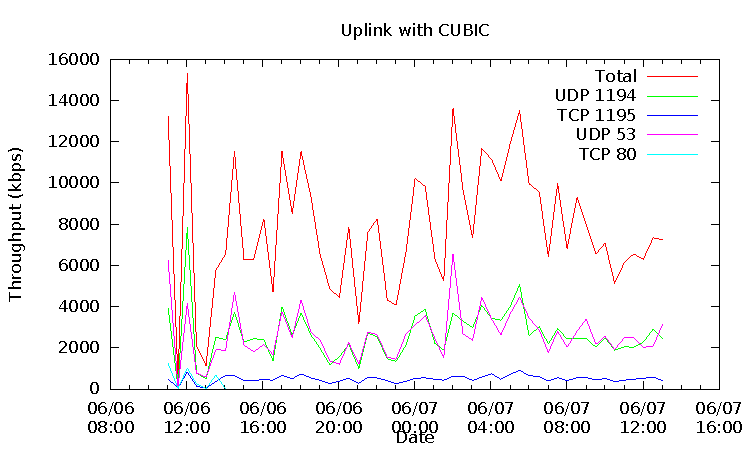
\includegraphics[width=0.75\textwidth]{img/up-cubic}
  \caption{Uplink with CUBIC}
  \label{fig:up-cubic}
\end{figure}

In terms of download performance, peak values are lower than upload, reaching
a maximum of 8Mbps, as can be observed in \ref{fig:down-cubic}. The average
value leans towards 4Mbps, same as the baseline. It is worth noticing that there
is a predilection for higher throughput values between 01:00 and 06:00. This
makes sense as normal users are sleeping during these hours and there is less
contention for the communication channel.

\begin{figure}[H]
  \centering
  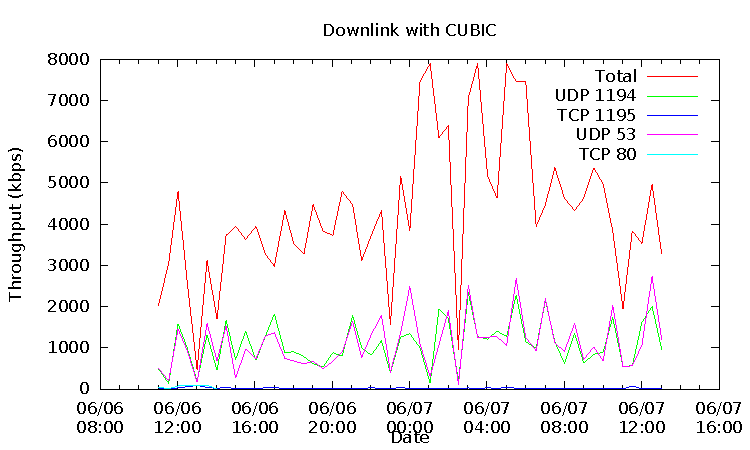
\includegraphics[width=0.75\textwidth]{img/down-cubic}
  \caption{Downlink with CUBIC}
  \label{fig:down-cubic}
\end{figure}

An aspect worth considering is that 3 hours into the tests, the HTTP tunnel
has ceased to contribute towards the total throughput. This could indicate the
fact that Operator 1 has blocked our OpenVPN traffic based on deep packet
inspection. We have not delved deeper into the manner and therefore cannot
provide a definite explanation, but it is certainly an anomaly warranting
further investigation.

Moving on to OLIA, a congestion control algorithm geared towards multipath
flows, we will contrast it with CUBIC. Looking at the upload throughput
outlined in \ref{fig:up-olia} the peaks value is slightly higher, namely
16Mbps. The average value is also higher, close to 10Mbps. The previouly
mentioned time intervals for poor performance seen with CUBIC are not
discernible.

\begin{figure}[H]
  \centering
  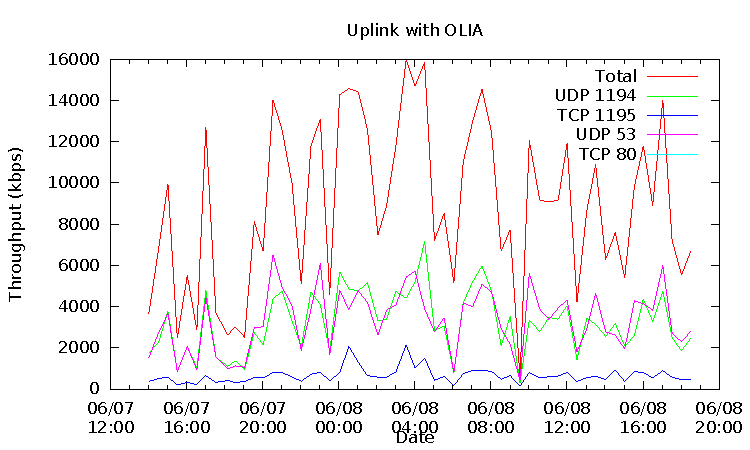
\includegraphics[width=0.75\textwidth]{img/up-olia}
  \caption{Uplink with OLIA}
  \label{fig:up-olia}
\end{figure}

When looking at download performance in \ref{fig:down-olia}, it can be noticed
immediately that we are dealing with reduced stability, as values between
successive tests can vary greatly. Peak and average values are lower than the
ones noticed for CUBIC. However, the tendency for higher throughput values
during night hours is similar to CUBIC.

\begin{figure}[H]
  \centering
  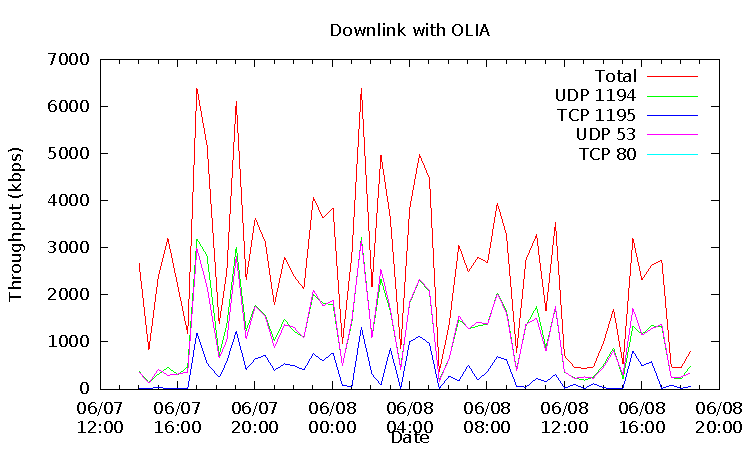
\includegraphics[width=0.75\textwidth]{img/down-olia}
  \caption{Downlink with OLIA}
  \label{fig:down-olia}
\end{figure}

The HTTP tunnel has not contributed in any way to the total throughput. Since
the OLIA tests have been run immediately after the CUBIC batch, we interpret
this as a direct consequence of the operator's aggresive blocking based on
deep packet inspection.
\begin{savenotes}
\begin{center}
	\begin{table}[htb]
	\centering
	\begin{tabular}{ | l | l | l | l | l | }
	\hline
	& UDP (1194) & TCP (1195) & DNS (53) & HTTP (80) \\ \hline
	CUBIC & 45.75\% & 8.88\% &  45.37\% & 0\%\footnote{During the small time frame it was active, the HTTP tunnel contributed roughly 1\% of the throughput and the contribution of the TCP tunnel was slightly reduced.} \\ \hline
	OLIA & 46.77\% & 7.74\% & 45.49\% & 0\% \\ \hline
	\end{tabular}
	\caption{Contribution of each tunnel towards total throughput}
	\label{table:iodine}
	\end{table}
\end{center}
\end{savenotes}

\section{IP-over-DNS tunneling with Iodine}

In order to gain a better understanding of how cellular network operators
perform traffic shaping on port 53 we have run a separate series of throughput
tests using Iodine. Iodine is an open source tool that allows tunneling IPv4
traffic through a DNS server. It is targeted at the scenario where Internet access is firewalled but DNS queries are allowed.

The experimental setup consists of the same Galaxy Nexus I9250 phone running a
cross-compiled instance of the Iodine client and an external server with a
public IP address running the Iodine server. Iodine creates  a tunnel interface called \textit{dns0} over which the server and the client can communicate by placing data inside DNS queries. The tests we perform include:

\begin{itemize}
\item UDP upload, using iperf with default parameters
\item TCP upload, using iperf with default parameters
\item HTTP download, using wget to download a file of 10 MB
\end{itemize}

We run three batches of the tests described above:

\begin{itemize}
\item using Iodine over the \textit{dns0} tunnel interface
\item using OpenVPN over port 53
\item using the default 3G interface \textit{rmnet0} with no tunnels for baseline comparison
\end{itemize}


\begin{center}
	\begin{table}[htb]
	\centering
	\begin{tabular}{ | l | l | l | l | l | }
	\hline
	& TCP up (Mbps) & UDP up (Mbps) & UDP dgram loss (\%) & HTTP down (Mbps) \\ \hline
	Baseline & 1.15 & 1.39 &  0.11 & 2.5 \\ \hline
	Iodine & 1.14 & 1.32 & 2.6 & 2.35 \\ \hline
	OpenVPN & 0.087 & 0.55 & 49 & N/A \\ \hline
	\end{tabular}
	\caption{Throughput comparison between Iodine, OpenVPN and default 3G. Average of ten tests run during daytime hours.}
	\label{table:iodine}
	\end{table}
\end{center}
	
Table \ref{table:iodine} presents the results. The 3G interface offers a low
throughput to begin with but Iodine manages to almost match it. The throughput
obtained by Iodine is consistent with documentation. It is also worth noting
that the Iodine tunnel is not affected by the packet losses we observe when
using OpenVPN. Port 53 traffic shaping is once again observed in the case of
OpenVPN:

\begin{itemize}
\item TCP throughput is very low. Only three out of ten tests finished. Packet captures on the server revealed only a handful of packets had arrived.
\item UDP traffic reveals a datagram loss of 49\% which affects throughput.
\item HTTP downloads using wget were unable to complete. The application repeatedly stalled after only a few kilobytes had been transferred.
\end{itemize}

Since Iodine was not affected by traffic shaping in the way OpenVPN was we can
conclude that Operator 1 differentiates between packets sent on port 53 and
actual DNS queries (inside of which Iodine hides the useful data). Therefore we can conclude that shaping is done not only based on destination port but also on packet type and content.
